
\begin{center}\texttt{5 - Cost Prediction}\end{center}
\hrulefill \\

\noindent You want to make a reliable assessment especially in the case of BRUF project: unlike in Agile, you cannot adjust the shot iteratively, it's important that a rough estimation is provided upfront;\\Unlike other engineering domains, software is tricky when it comes to predict the cost, same usual reason being that it's not a physical good. Factors that can contribute to the difficulty of cost predictions include:
\begin{itemize}
    \item requirements are unclear $\rightarrow$ be very careful when defining those!;
    \item costs dominated by human labour (man-months) $\rightarrow$ make sure to predict the costs and changes of those;
    \item sources of uncertainty;
    \item outsourcing parts of the prj (relinquish the work to someone external), reuse of parts;
    \item subjective nature: we tend to underestimate small prjs, and overestimate big prjs;
    \item different past experience will lead different people to give different cost estimations.
\end{itemize}

\noindent As you work on the prj, time available decreases and your knowledge increases. Throughout the various phases of the prj's life cycle, you should have more accurate estimations.

\noindent Brooks' Law: putting more people on a late job makes it later.

\noindent Techniques to derive estimation of sw cost:
\begin{itemize}
    \item Delay estimation til later in the prj - the more you can delay, the more accurate (if grandpa had 3 testicles he would've been a Pinball arcade);
    \item Use composition techniques (those we considered during planning, WBS and activity identification and allocation... or PBS). You just compute the effort based on people working on the prj;
    \item Use empirical models (like COCOMO-II);
    \item Make an estimation based on similar completed prjs;
    \item expert judgement;
    \item Price to Win and Parkinson's law. P2W is about beating the alternative product by making it more convenient. Base the analysis on the fact that you want to win that race (careful not to overdo it). Avoid these, they result in cutting on reqs, activities, testing, and thus lose quality;
\end{itemize}
\noindent You might want to use more than one technique to make sure that the results are pretty similar. If they are very different you might ask yourself what's going on.

\[ Effort = systemSize \times productivityRate\]

\noindent Many techniques are based on the concept of effort and these two parameters. The higher the prodRate, the lower the required effort, bc the staff is able to do a lot of stuff in a certain time lapse - it's the ratio between units produced in T divided by the nr of person hours required. The size of the prj can be considered from different perspectives: function-related metrics (requirements-related), size-related metrics (LOCs and such).

\noindent  The LOCs we take into consideration are supposedly correct LOCs, which means they've also been tested, accepted in the final version of the system. Cost is Effort $\times$ Salary. Plus an overhead that depends on the company (upon financial assessment, think heating, lighting of the office... side costs).

\noindent Measure functionalities: Albrecht FP analysis, classify the functionalities you have and then try to identify how many of them of each class you have in your software. This is closer to requirements than the strict LOC approach, it's more accurate.

\noindent Function Point analysis in 4 steps:
\begin{enumerate}
    \item identify functions, through keywords such as \textit{retrieve, display...} It's rather complex. The IFPUG has recommendations on how to identify F's;
    \item try to assign points to each FP based on its contribution:
    \begin{itemize}
        \item external inputs EI: assign a point for each individual input that can affect the functionality;
        \item external outputs EO: assign a point for each output that leads to non trivial computation;
        \item external inquiry EQ: assign a point for each result of query, just query, retrieving data;
        \item internal logical files ILF: assign a point for each unique group of data maintained by the application (i.e., the app is responsible for deriving storing data);
        \item external logical files ELF: like a JSON, assign a point for each unique logical group of data on system external to the app - the complexity of data that can be transferred.
    \end{itemize}
    \item collect historical data, split the points in each category into 3 disjoint group of Low, Average, High complexity; the sum of all those is called the UFP: unadjusted FP;
    \item considering external factors, establish the impact that each factor may have on your project, from 0 = None to 5 = Essential. These are 14 factors that answer these questions (GC):
    
    \begin{figure} [H]
        \centering
        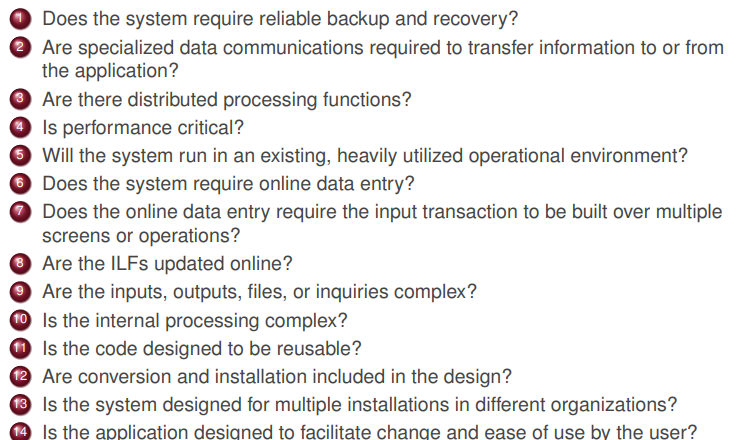
\includegraphics[width=0.75\linewidth]{Figures/05/fp1.png}
    \end{figure}

\item compute the adjusted FPs as follows:
\[FP = UFP \times (0.65 + 0.01 \times \Sigma(GC_i))\]
Where $GC_i$ is the value of the $i$-th General Characteristics.
\end{enumerate}

\noindent Object Points: different approach, object-oriented. Instead of Functions and FPs we have Objects, OPs can be computed by complexity of each screen, or number of produced reports etc., relevant aspects in general.

\noindent Another alternative is to base the estimation on Use Cases - which can be reconnected to LOCs through:

\begin{figure} [H]
    \centering
    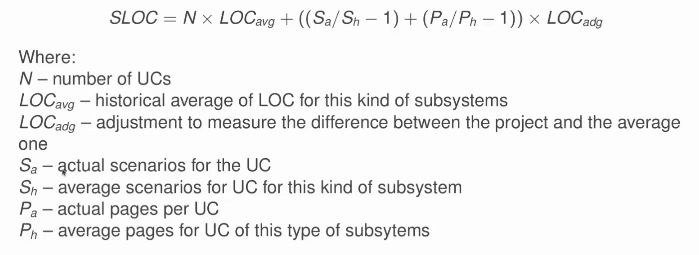
\includegraphics[width=0.75\linewidth]{Figures//05/locOP.png}
\end{figure}

\noindent You get the average LOCs, then you adjust it depending on the complexity of the use cases you have. The downside of UC based estimation is that UCs can come in very different styles based on who develops them, plus it's complex to estimate costs when external systems are involved, you don't see that complexity in a line of a Use Case. 

\noindent You can make an estimation based on experts' opinion, similarly to the activity planning, optimistic average pessimistic estimation...

\noindent Decomposition: estimate costs of subsystems! Then recompose the system and thus the costs.

\noindent Wolverton strategy: based on complexity, functionality but also similarities, there's the concept of novelty for functions.

\noindent Process based estimation: once you identify the activities, make an assessment in terms of effort in PMs for each activity. Activity evaluation is based on the optimal allocation of resources (think moving the chair in the room).

\noindent Algorithmic cost modelling: effort is encoded in a formula:
\[E = (a+bS^c)m(X)\]

\noindent a, b, and c are constants defined from empirical studies, S is the size of the product (according to some metric), m is a multiplier, X is a vector of many factors. 

\begin{figure} [H]
    \centering
    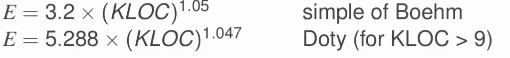
\includegraphics[width=0.75\linewidth]{Figures//05/cost1.png}
\end{figure}

\noindent COCOMO: empirical model for waterfall process and imperative prog Language

\begin{figure} [H]
    \centering
    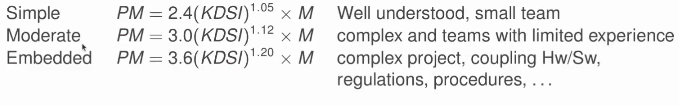
\includegraphics[width=0.75\linewidth]{Figures//05/cocomo1.png}
    \caption{COCOMO formulae based on project complexity}
\end{figure}

\noindent COCOMO-II: adapts to newer products, languages and techniques. It has sub-models you can apply on your project based on which stage your prj is in.

\noindent Application composition model: use it when your system has reusable components, scripting or db programming, or prototype development (early stage! rough assessment).
\begin{figure} [H]
    \centering
    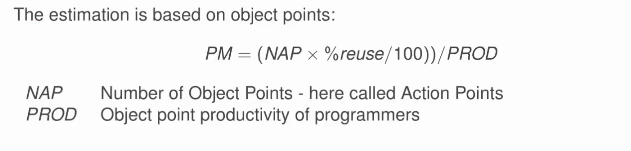
\includegraphics[width=0.75\linewidth]{Figures//05/cocomo2acm.png}
    \caption{Effort estimation for Application Composition Model sub-model.}
\end{figure}

\noindent Early design model: you're at the beginning of the prj, so you have a more or less accurate idea of the requirements of the system.

\begin{figure} [H]
    \centering
    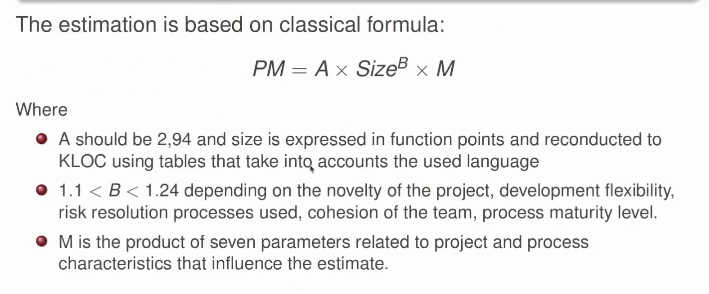
\includegraphics[width=0.75\linewidth]{Figures//05/cocomo2edm.png}
    \caption{Effort estimation for Early Design Model}
\end{figure}

\begin{figure} [H]
    \centering
    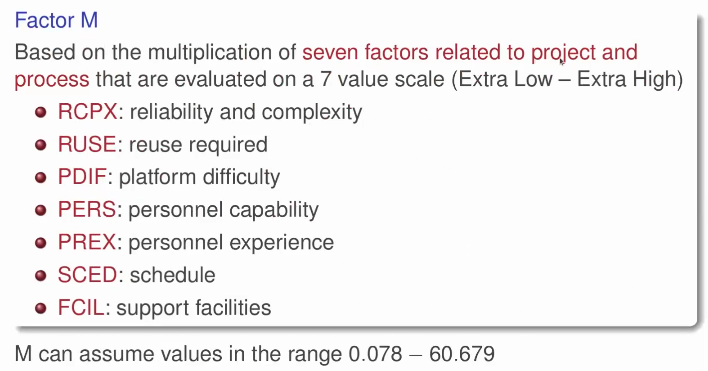
\includegraphics[width=0.75\linewidth]{Figures//05/cocomo2edm2.png}
\end{figure}

\noindent Reuse model: for systems based on reusable components and automatically generated code. Base the estimation on what percentage of code you can reuse or automatically generate

\begin{figure} [H]
    \centering
    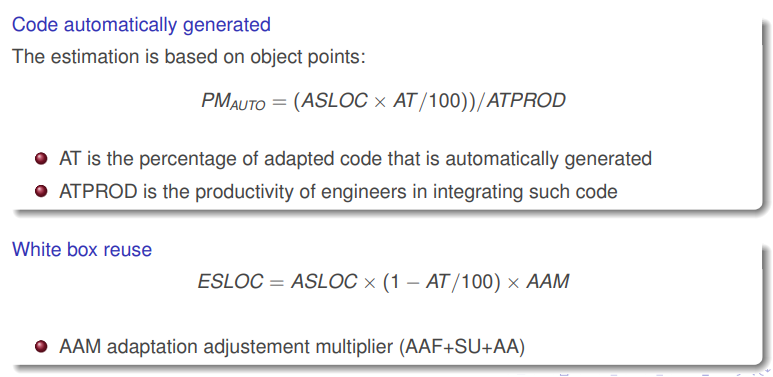
\includegraphics[width=0.75\linewidth]{Figures//05/cocomo2reuse.png}
    \caption{Effort estimation for reuse model. White box reuse means you're reusing code and you also have access to it.}
\end{figure}

\noindent Post-architecture model: the system architecture is available now. The formula is the same as the early design model but now M considers 17 factors, it is much more complex!. B depends on factor such as previous experience of the organization, dev flex, architecture/risk resolution, team cohesion, process maturity, and each has an attribute from very low to very high. You want to ask yourself which factors are relevant to you and your project.

\noindent 